% Complete project explanation — written to be the source material for slides and for the dissertation.
\documentclass[11pt,a4paper]{article}
\usepackage[margin=2.3cm]{geometry}
\usepackage{graphicx}\usepackage{booktabs}\usepackage{xcolor}\usepackage{titlesec}
\usepackage{enumitem}\usepackage[hidelinks]{hyperref}\usepackage{helvet}\usepackage{parskip}
\usepackage{tcolorbox}\usepackage{longtable}
\renewcommand{\familydefault}{\sfdefault}

\definecolor{ink}{HTML}{1D2227}\definecolor{blue}{HTML}{31708F}\definecolor{gold}{HTML}{B07D2B}
\definecolor{soft}{HTML}{5A636C}\definecolor{green}{HTML}{3C7A4E}\definecolor{red}{HTML}{9E3B33}
\definecolor{wash}{HTML}{EEF3F6}

\titleformat{\section}{\Large\bfseries\color{ink}}{\thesection}{0.7em}{}
\titleformat{\subsection}{\large\bfseries\color{blue}}{\thesubsection}{0.6em}{}
\setlist{nosep,leftmargin=1.3em}
\newtcolorbox{key}[1][]{colback=wash,colframe=blue,boxrule=0.6pt,left=8pt,right=8pt,top=6pt,bottom=6pt,#1}
\newcommand{\say}[1]{\textit{\color{soft}#1}}

\begin{document}

\begin{center}
{\Huge\bfseries Visualising Emotion}\\[8pt]
{\Large How far does an automatic reading of an AI drawing agree with an automatic reading of the words that made it?}\\[14pt]
{\color{soft}\large A complete explanation of the project}\\[10pt]
{\color{soft}MSc Artificial Intelligence dissertation · Shre Hari Prem Anandh}\\
{\color{soft}Supervisor: Dr Chaona Chen · University of Sheffield}\\[4pt]
{\color{soft}\small Every figure in this document was re-verified against the analysis on 9 September 2026}
\end{center}
\vspace{6pt}\hrule\vspace{12pt}

\begin{key}
\textbf{The project in one paragraph.} At the Festival of the Mind 2024, members of the public typed a
few words about how they were feeling, and DALL$\cdot$E drew each entry as a black-and-white line
drawing --- 1{,}025 records; the number of contributors is unknown. This project builds and validates a
way to measure how far an automatic reading of the drawing agrees with an automatic reading of the
words. It finds that agreement is real and well above chance where the describer reports a readable face
--- and, once the description stops inventing an expression, at chance where it reports a scene ---
that the same words do not reliably give the same reading, and that the method used to measure it
matters a great deal.
\end{key}

\section{The question}

You can already check whether an AI drew what a prompt asked for, provided the prompt names objects.
Ask for \say{a red car} and a metric can look for a car and check that it is red. That is what most
text-to-image evaluation does.

Feelings do not work that way. If somebody types \say{tired but happy}, there is no object to look
for. There is no agreed answer key. And the feeling is mixed, which most emotion tools handle badly.

\begin{key}
\textbf{The precise question this project answers:}\\[4pt]
To what extent does an automatic image-emotion reader agree with prompt-derived emotion labels for
AI-generated monochrome drawings, and how does that agreement vary by visual content and by repeated
prompts?
\end{key}

That wording matters, and it is deliberately narrower than \say{does the drawing convey the
feeling}. This project measures \textbf{agreement between two automatic systems} — one reading the
words, one reading the drawing. It does not establish that a human viewer perceives the same
feeling. That distinction is carried honestly through everything that follows.

\section{Why the question is open}

97 papers were collected, read and triaged; 24 were excluded and 73 kept as core evidence, organised
into eight themes. The literature establishes four things that, taken together, leave a gap.

\begin{itemize}
\item \textbf{Emotion in text is well studied.} GoEmotions supplies a 28-label taxonomy (27 emotions plus
neutral), a large labelled corpus and an off-the-shelf classifier. But short, first-person self-report is the hardest
register for these tools, and free self-report resolves roughly 27 blended categories rather than a
tidy handful.
\item \textbf{Emotional image \emph{generation} is well studied.} Systems exist that generate images
towards a chosen target emotion. Alvarado (2025) finds that in text-to-image output lightness and
chroma, rather than hue, are the principal colour carriers of emotional meaning; that study models
colour features only, so it gives no evidence either way about whether form and line can do the same.
\item \textbf{Text-to-image \emph{evaluation} is well studied, but for objects.} The metrics score
whether the picture contains what the prompt named. Recent work shows these metrics are fragile
enough to be flipped by small perturbations.
\item \textbf{Reading emotion back out of an image is possible but weak.} Vision-language models are
positively biased and order-sensitive readers of emotion.
\end{itemize}

\begin{key}
\textbf{The gap.} Within the 73-paper corpus reviewed here, no work measures prompt-reader /
image-reader agreement for short, unmediated, mixed-affect first-person self-reports rendered as
monochrome line art, nor the stability of that reading under repeated prompts. This dataset is
unusually well suited to asking: the prompts are real, first-person, short and often mixed; and
because the drawings are monochrome line art, the channel the literature says usually carries
emotion --- colour --- is simply absent.
\end{key}

\textbf{An important restraint.} The colour literature motivates why this dataset is a hard case. It
is \emph{not} a result of this project. There is no colour-control condition here, so no claim is
made about the effect of removing colour. Every finding applies within this monochrome corpus.

\section{The dataset, and what it took to use it}

\begin{center}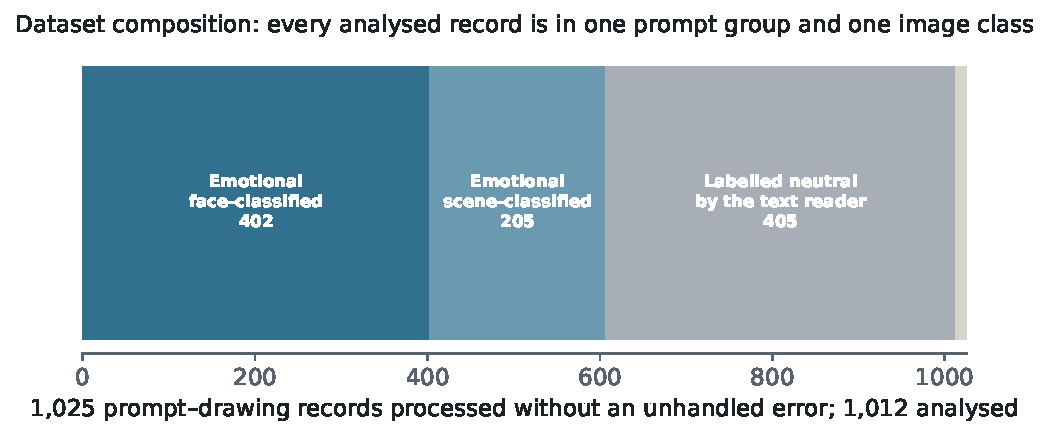
\includegraphics[width=0.95\textwidth]{../../../emoviz/outputs/figures/fig5_dataset.pdf}\end{center}

1,025 prompt--drawing records. Median prompt length is about four words. Visitors were invited to
describe how they were feeling but the interface accepted free text, so a substantial minority of
entries are object or scene requests rather than self-report. Records are not linked to individuals
and 249 repeat an earlier prompt, so the number of contributors is unknown and no greater than 763.
Before any analysis, three properties had to be handled.

\begin{itemize}
\item \textbf{Three incompatible filename schemes} in one folder: \texttt{img\_00001.PNG} for ids
1--199, \texttt{img\_200.PNG} for 200--999, \texttt{img\_t1000.PNG} for 1000 and above --- and two
files use a lowercase extension. A naive loader resolves under 20\% of the corpus; the loader written
here resolves 100\%.
\item \textbf{Hidden provenance metadata.} Every PNG carries a C2PA/JUMBF manifest containing an
RFC-3161 signing timestamp. Recovering it gave a creation time per image and revealed that
\textbf{records 1--13 were generated before the festival} --- developer tests. They are processed but
excluded from analysis, so nothing is silently dropped.
\item \textbf{Repeated prompts.} 87 distinct prompts were drawn more than once, covering 336 records
(43 of the groups are pairs). This looked like a nuisance and became a finding.
\end{itemize}

\begin{center}
\begin{tabular}{@{}lr@{}}
\toprule
\textbf{Dataset accounting} & \textbf{Records}\\
\midrule
Processed by the pipeline (no unhandled errors) & 1{,}025\\
Pre-festival developer tests, excluded & 13\\
\textbf{Analysed} & \textbf{1{,}012}\\
\quad prompts the text reader labels emotional & 607\\
\quad prompts the text reader labels neutral (the specificity set) & 405\\
\quad face-classified (describer reports a person and an expression) & 591\\
\quad scene-classified & 421\\
Distinct prompts (identity from pre-redaction text) & 763\\
Records repeating an earlier prompt & 249\\
\bottomrule
\end{tabular}
\end{center}

\section{The method}

The supervisor's instruction was decisive: \textbf{never ask a vision model what emotion a picture
shows.} Describe the picture in plain factual terms, then infer the feeling from that description
with a separate model. The pipeline implements exactly that.

\subsection{Stage by stage}

\begin{enumerate}
\item \textbf{Load and redact.} Prompts are loaded through a single loader that applies name
redaction, so the analysis, the figures and the demo app cannot diverge.
\item \textbf{Describe.} BLIP-VQA is asked five fixed questions about the drawing: \say{What is the
facial expression?}, \say{What is the person doing?}, \say{What is the body posture?}, \say{How many
people are there?}, \say{What is in the picture?} The answers are assembled into one neutral
sentence. \textbf{The word ``emotion'' never appears in any question} --- though the expression
question returns a bare emotion word for 41\% of records, and where it does the next stage follows
it 99.8\% of the time (see Limitations).
\item \textbf{Extract, image side.} A zero-shot natural-language-inference model reads that
description against the hypothesis template \say{This scene conveys \{\}.} across seven emotion
families, returning a ranked distribution.
\item \textbf{Extract, text side.} GoEmotions reads the person's own words, and its 28 labels are
collapsed onto the same seven families, so both sides live in one label space.
\item \textbf{Compare.} Four similarity measures, each referenced to chance.
\end{enumerate}

\subsection{Models used}

\begin{center}
\begin{tabular}{@{}llp{5.6cm}@{}}
\toprule
\textbf{Model} & \textbf{Size} & \textbf{Role}\\
\midrule
\texttt{Salesforce/blip-vqa-base} & $\sim$385M & Describes the drawing (five questions)\\
\texttt{facebook/bart-large-mnli} & $\sim$407M & Reads a feeling from that description\\
\texttt{SamLowe/roberta-base-go\_emotions} & $\sim$125M & Reads a feeling from the person's words\\
\midrule
OpenCLIP ViT-B/32 (LAION-2B) & $\sim$151M & \emph{Frozen baseline only} --- the older
``ask CLIP directly'' method, kept for comparison\\
\bottomrule
\end{tabular}
\end{center}

\subsection{The four similarity measures}

Similarity, not matching --- \say{happy} and \say{excited} should count as close, not as a miss.

\begin{enumerate}
\item \textbf{Valence--arousal similarity.} Each side's ranked emotions are collapsed to a single
point on a pleasantness/energy plane using fixed centroid coordinates per emotion, and the measure is
one minus the normalised distance between the two points. \emph{This is a designed proxy built on
hand-set centroids, not a continuous lexicon rating.}
\item \textbf{Valence-sign agreement.} Do both sides land on the same side of pleasant/unpleasant?
\item \textbf{Emotion-family agreement.} Do both sides pick the same emotion family outright?
\item \textbf{Top-3 overlap.} How much of the two ranked distributions actually coincides?
\end{enumerate}

\section{What was tried and rejected}

Each link was tested before being trusted. The failures shaped the design and are findings in their
own right.

\begin{center}
\begin{tabular}{@{}p{4.9cm}p{9.3cm}@{}}
\toprule
\textbf{Approach} & \textbf{Why it was rejected (evidence)}\\
\midrule
GoEmotions on the image descriptions & Collapses to \emph{neutral} above 0.95. It is trained on
first-person feeling words; a third-person visual description contains none.\\
A single BLIP caption fed to the reader & Captions too terse (\say{a man with hands in the air});
the reader collapses to \emph{surprise} for almost everything.\\
BART-MNLI on the \emph{prompt} side & Over-reads \emph{surprise} on short first-person text: 333 of
1{,}025 prompts came back as surprise. GoEmotions used instead.\\
Qwen2.5-VL-3B as the describer & 7\,GB in half precision exceeded a 16\,GB laptop; thrashed into
swap with \textbf{zero progress after 4\,h\,45\,min}. Never produced a description.\\
Florence-2 as the describer & Hard library incompatibility (\texttt{forced\_bos\_token\_id}) on
transformers 5.14.\\
Asking CLIP directly for the emotion & Agreed far less with the prompt reader in the like-for-like
comparison (see Findings), and manual inspection found clear errors: arms-raised celebration read as
\emph{anger} 0.73.\\
\midrule
\textbf{BLIP-VQA (chosen)} & $\sim$0.4B, roughly 1.5\,s per record, and its ``facial expression''
answer supplies exactly the affective cue the next stage needs.\\
\bottomrule
\end{tabular}
\end{center}

\section{How the numbers are kept honest}

This is the part that makes the findings usable, and it is where most of the methodological effort
went.

\subsection{A random-pairing null for every metric}

Within each subset, the image side is shuffled and re-paired against the untouched prompt side, and
all four metrics are recomputed. This is repeated \textbf{300 times} with a fixed seed. The average
is the chance level; the spread gives a $z$-score. Every number reported in this project is quoted
against its own null. A result counts only insofar as it beats chance.

\subsection{A specificity check}

\begin{center}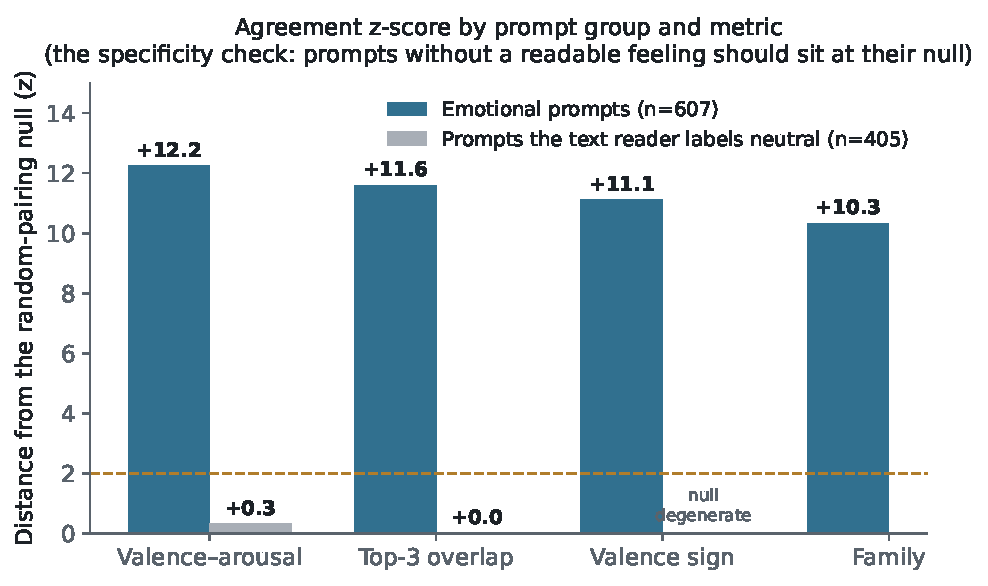
\includegraphics[width=0.78\textwidth]{../../../emoviz/outputs/figures/fig3_z_by_prompt_group.pdf}\end{center}

405 of the 1{,}012 prompts are labelled neutral by the text reader --- \say{pigs}, \say{mickey mouse},
\say{disney characters}. If the method were finding agreement where the prompt side has no readable
feeling, it would score above chance on these. Only the valence--arousal measure is informative here:
76.6\% against a null of 76.6\%, $z=+0.3$. Valence-sign and family agreement are degenerate on this
subset --- every prompt shares the neutral label, so permutation cannot change them and their $z$ is
zero by construction, not by measurement. Two caveats: 68 of the 405 (16.8\%) contain a plain affect
word (calm, content, tired, relaxed, stress), and two consist of a name alone; on the cleaned 335 the
$z$ is $+0.04$, still at the null. The set is therefore better described as ``prompts the text reader
could not read affect from'' than as prompts with no feeling.

\begin{key}
\textbf{Why this matters.} An instrument that reported a signal where the prompt side has none could
not be trusted anywhere. This check, resting on one measure, is one reason --- not the only one ---
that the other numbers can be read.
\end{key}

\subsection{A robustness check on repeated prompts}

249 records repeat an earlier prompt, so treating all 1{,}012 as independent would overstate
confidence. Every headline was re-run on the 763 distinct prompts (452 emotional). The overall and
face results are essentially unchanged ($z$ $+9.3$ to $+10.8$; face valence-sign 71.8\%, $z{+}8.4$).
The scene result weakens substantially (valence-sign 37.3\%, $z{+}3.5$; family 30.8\%, $z{+}2.6$, $n$
falling from 205 to 133), and its family $z$ does not survive a Holm--Bonferroni correction across the
36 non-degenerate $z$-scores (26 survive at family-wise 0.05).

\subsection{Degenerate nulls are refused --- automatically}

Where a subset shares one label by construction --- for example the neutral-labelled records ---
shuffling cannot change the score, so the ``null'' is an identity rather than a baseline. The
analysis detects this from the null's own spread (zero standard deviation) and prints no $z$ for such
a measure: the sign measure on the single-valence subsets, the family measure on the positive-prompt
subset, and both on the neutral-labelled subset. The negative-prompt family null is not degenerate.

\subsection{Confidence intervals, and a test of the difference}

Every reported rate carries a 95\% confidence interval from a clustered bootstrap (10{,}000 draws,
resampling prompt groups rather than records, because 249 records repeat an earlier prompt). The
face/scene difference is tested directly with a clustered permutation test (10{,}000 draws):
$+30.9$\,pp [$+22.6$, $+40.6$] for valence sign and $+26.3$\,pp [$+18.4$, $+35.3$] for family,
$p = 0.0001$ for both. Cohen's $\kappa$ for family agreement is 0.23 [0.18, 0.29] on the emotional
prompts, 0.30 [0.23, 0.37] face-classified and 0.13 [0.06, 0.19] scene-classified --- fair, fair and
slight. After a Holm--Bonferroni correction across all 36 non-degenerate $z$-scores, 26 survive; the
ten that do not are the control cells, the single-valence valence--arousal and overlap cells, and the
distinct-prompt scene family result.

\section{Chance is not zero}

A late and important discovery, which changed how results are reported.

\begin{key}
The valence--arousal similarity measure \textbf{cannot fall below 41\%} --- that is its mathematical
floor, given the fixed emotion coordinates. Two \emph{randomly paired} records already score about
\textbf{76--77\%}, because most emotions sit close together on the plane.\\[6pt]
So a score of 71\% looks like a pass and is in fact \textbf{below chance}. On a bare 0--100 scale
that is invisible.
\end{key}

There is a second consequence. That measure returns roughly 84\% for face drawings and 83\% for
scene drawings --- it cannot tell them apart. The face/scene difference lives in valence-sign and
emotion-family agreement. The reporting was changed accordingly: those two measures lead, and the
valence--arousal score is always shown against its measured chance line.

\section{Findings}

\subsection{Agreement is real, and much stronger where the describer reports a face}

\begin{center}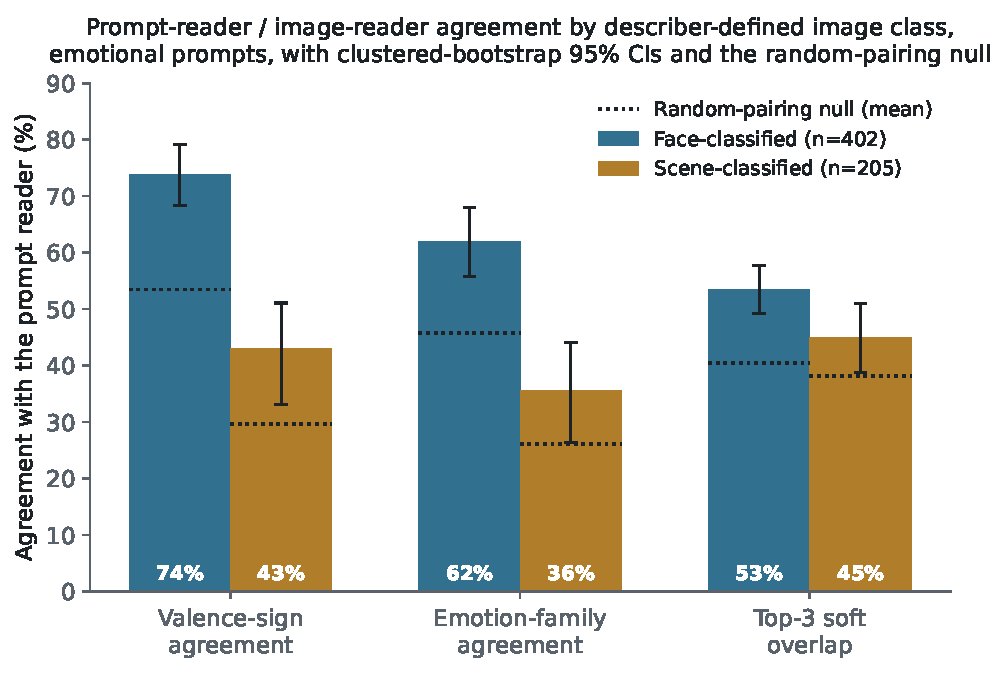
\includegraphics[width=0.9\textwidth]{../../../emoviz/outputs/figures/fig1_face_vs_scene.pdf}\end{center}

\begin{center}
\begin{tabular}{@{}lccc@{}}
\toprule
\textbf{Emotional prompts only} & \textbf{Valence sign} & \textbf{Emotion family} & \textbf{Top-3 overlap}\\
\midrule
Face drawings ($n=402$)  & \textbf{73.9\%} ($z{+}10.4$) & \textbf{61.9\%} ($z{+}10.3$) & 53.4\% ($z{+}11.6$)\\
Scene drawings ($n=205$) & 42.9\% ($z{+}5.8$) & 35.6\% ($z{+}4.4$) & 44.9\% ($z{+}4.9$)\\
\midrule
All emotional ($n=607$)  & 64.0\% ($z{+}11.1$) & 53.0\% ($z{+}10.3$) & 50.6\% ($z{+}11.6$)\\
\bottomrule
\end{tabular}
\end{center}

Both are above their nulls (95\% intervals: face valence-sign [68.3, 79.2], scene [33.1, 51.1]).
The difference is $+30.9$\,pp [$+22.6$, $+40.6$] for valence sign and $+26.3$\,pp [$+18.4$, $+35.3$]
for family, clustered permutation $p = 0.0001$. No ratio is quoted, because the two nulls differ. On
distinct prompts only the face result holds (71.8\%, $z{+}8.4$) while the scene result weakens
(37.3\%, $z{+}3.5$).

\textbf{Stated carefully:} the pipeline finds stronger prompt-reader / image-reader agreement for
drawings it \emph{classifies} as containing a readable face. It is not evidence about faces as such,
because the classification and the emotion reading share a source --- see Limitations. The template
ablation below shows the scene rows were an artefact of that shared source: described honestly,
scene-classified drawings give nothing above chance for this reader.

\subsection{The same words do not reliably give the same reading}

\begin{center}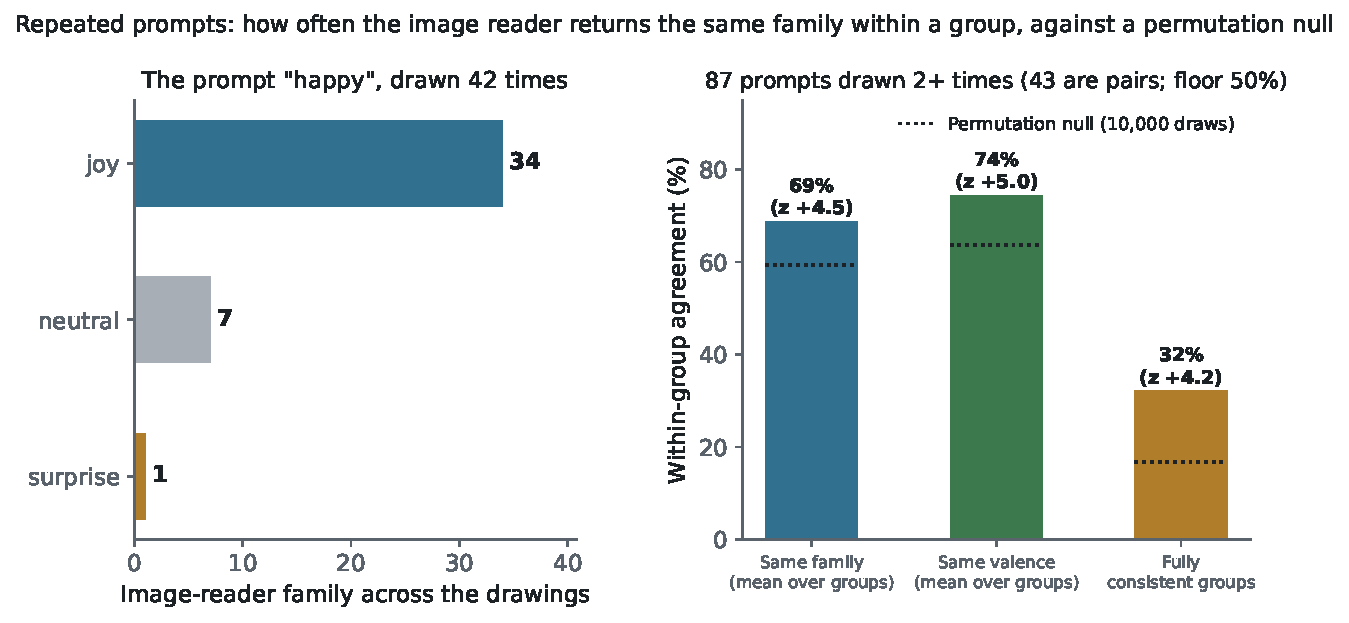
\includegraphics[width=0.92\textwidth]{../../../emoviz/outputs/figures/fig4_consistency.pdf}\end{center}

87 prompts were drawn between 2 and 42 times each, covering 336 records. Given \emph{identical}
words, the image reader returns the same family for \textbf{68.8\%} of the drawings within a group,
against a permutation null of 59.4\% ($z{+}4.5$, $p = 0.0001$; 10{,}000 draws), and \textbf{28 of
the 87} groups are fully consistent against 14.5 by chance ($z{+}4.2$). Half the groups are pairs,
whose modal agreement cannot fall below 50\%. The reading is more consistent than chance but far
from fixed --- and it measures the whole prompt$\rightarrow$image$\rightarrow$reader chain, not the
generator alone, since generation parameters were never recorded and the reader has no reliability
estimate of its own. A single drawing is one sample, not a fixed answer.

\subsection{The method matters: describe-then-extract agrees far more closely}

\begin{center}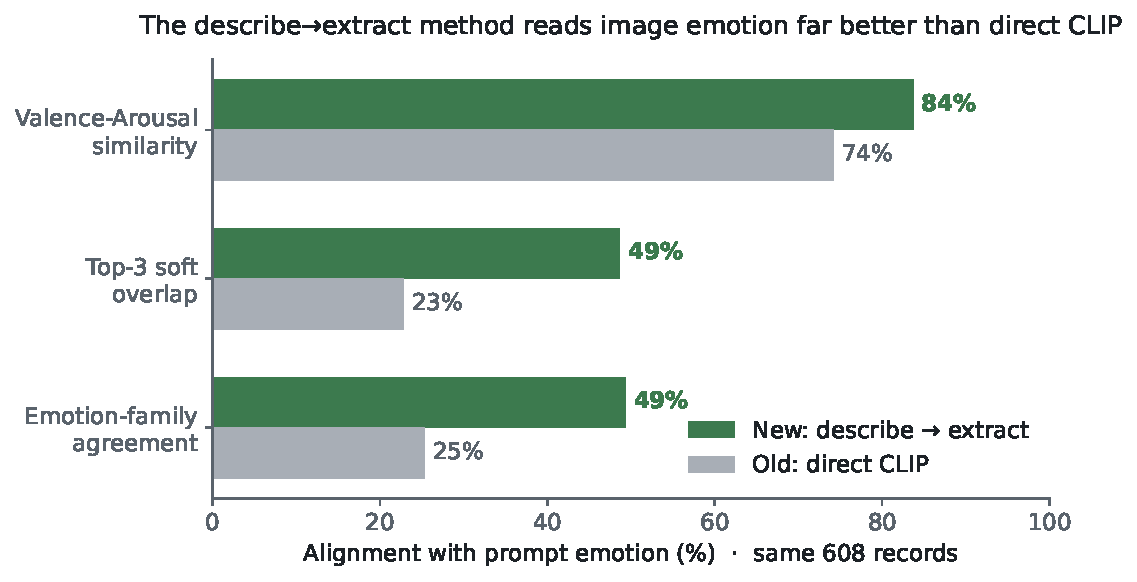
\includegraphics[width=0.88\textwidth]{../../../emoviz/outputs/figures/fig2_method_comparison.pdf}\end{center}

Like for like --- same GoEmotions prompt reader, same 607 emotional records, same measures, only the
image reader varied: describe-then-extract reaches \textbf{53.0\%} emotion-family agreement against
\textbf{22.4\%} for asking CLIP directly ($+30.6$\,pp; clustered 95\% interval [$+25.5$, $+35.6$];
cluster-level $p < 0.0001$), 64.0\% against 31.1\% on valence sign, and 50.6\% against 26.4\% on
top-3 overlap. Direct CLIP reads 283 of the 607 drawings as neutral. Neither reader has ground truth,
so this ranks two image readers against a third model's labels: they disagree, and describe-then-extract
is far closer to the text reader. The supervisor's redirection was supported rather than assumed. (The
earlier figure of 49.3\% against 25.3\%, on 608 records with the NLI prompt reader, is kept only as
the historical v1 record.)

\subsection{Where the readers disagree}

\begin{center}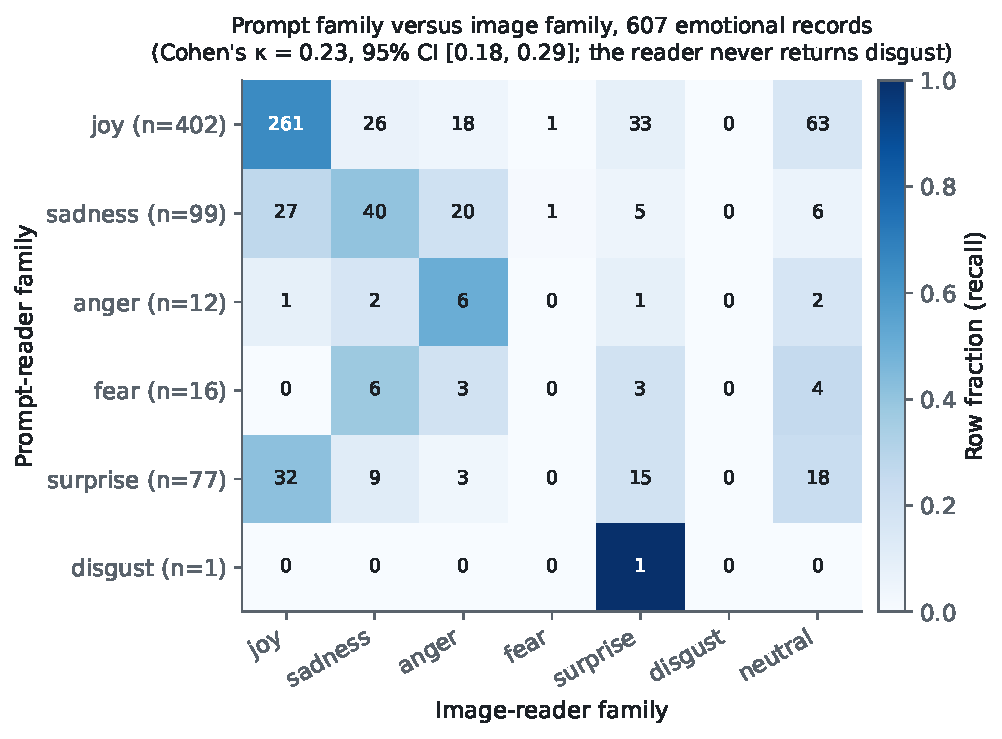
\includegraphics[width=0.8\textwidth]{../../../emoviz/outputs/figures/fig6_confusion.pdf}\end{center}

Three families are too rare on the prompt side to support family-level claims (fear $n=16$, anger
$n=12$, disgust $n=1$), and the image reader never returns disgust and returns fear four times across
all 1{,}012 records. Every high-confidence disagreement (both readers $\geq 0.8$, families differ: 38
records) was examined against the drawing and assigned a primary failure mode: 19 trace to the
describer (a face or expression invented, or read wrongly), 5 to the image reader, 12 to the prompt
side (ambiguous or mixed feelings), and 2 to a drawing that does not depict its prompt.

\subsection{What the reading rests on: the template ablation}

\begin{center}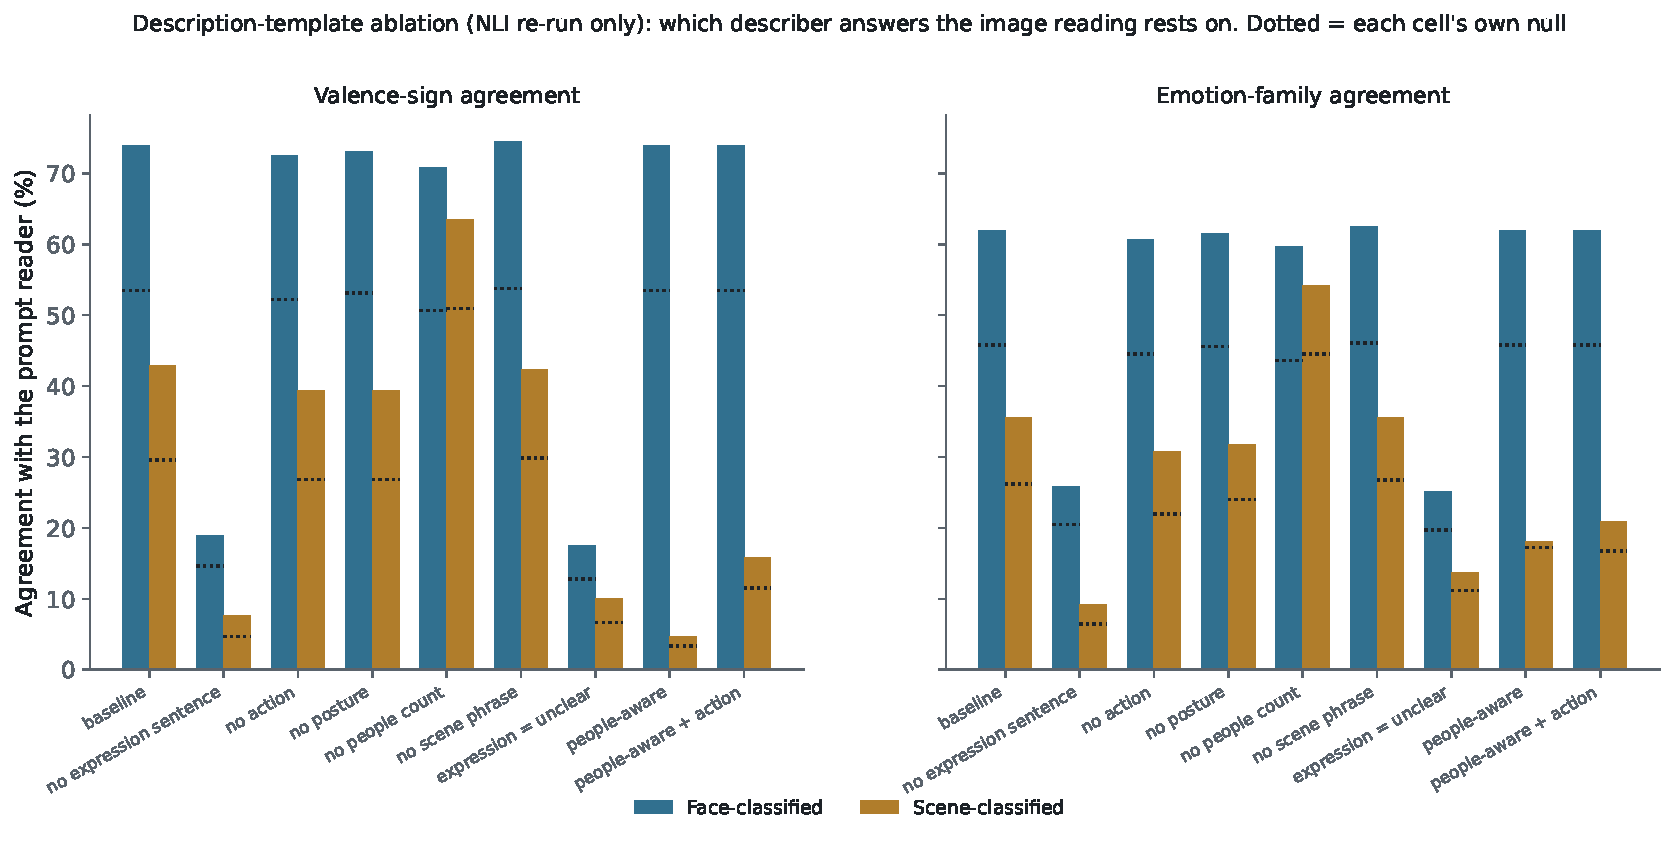
\includegraphics[width=0.95\textwidth]{../../../emoviz/outputs/figures/fig8_ablation.pdf}\end{center}

Each record's five cached describer answers were re-composed under an altered description template
and only the NLI stage re-run (\texttt{ablate\_nli.py}); a control re-run of the unmodified template
reproduces every baseline number exactly (0 of 1{,}012 top-1 readings change), so every difference is
a template effect. Removing the expression sentence collapses agreement --- all-emotional family
53.0\% $\rightarrow$ 20.3\% (null 16.6\%, $z{+}3.8$), valence sign 64.0\% $\rightarrow$ 15.3\% (11.4\%,
$z{+}5.1$); fixing the expression word to ``unclear'' gives the same collapse (family 21.3\%,
$z{+}3.9$), and the reader's output falls to surprise or neutral (514 and 368 of 1{,}012). Removing
the action, posture or scene clause moves the rates by 1--3\,pp. Removing the people count raises
rates and nulls together (scene valence sign 63.5\% vs 50.9\%, $z{+}5.0$): the ``0'' token pulls
scene readings toward neutral, and $z$ barely moves.

\begin{key}
Under a \textbf{people-aware template} --- \say{A drawing showing \{scene\}.} wherever the describer
reports no person, every other record unchanged --- the face rows are unchanged by construction
(73.9\% / 61.9\%) and \textbf{scene agreement falls to its null}: valence sign 4.7\% vs 3.4\%
($z{+}1.6$), family 18.0\% vs 17.3\% ($z{+}0.6$); keeping the action and posture clauses gives 15.9\%
vs 11.6\% ($z{+}2.7$) and 21.0\% vs 16.8\% ($z{+}2.2$). All-emotional under the people-aware
template: sign 51.7\% vs 36.9\% ($z{+}10.1$), family 47.1\% vs 34.5\% ($z{+}8.8$).
\end{key}

Four readings follow. (1) The image reading rests on one word --- the describer's expression answer
--- the same conclusion the 99.8\% copy rate reaches independently; in effect the pipeline is ``ask
the describer for the facial expression and map that word to a family''. (2) The scene result in
the headline table ($z{+}5.8$) was an artefact of the template asserting a person and an expression
for drawings with none; under an honest description this reader finds nothing above chance in
scene-classified drawings. (3) The face/scene contrast is therefore \emph{faces, and only faces, for
this reader}, not ``faces more than scenes''. (4) Whether scene drawings hold a feeling a person can
read is exactly what the human check tests; a scene-capable describer is the main further-work item.

\section{The demo application}

A small local web application runs the real pipeline live: choose a drawing from the dataset or
upload an image, see the five factual answers, see both emotion readings side by side, and see the
similarity scored against chance. It exists to make the method inspectable rather than to collect
anything.

Every number it shows is referenced to the measured chance line: the axis starts at the metric's real
floor of 41, the middle half of random pairings is bracketed, and the headline reads \say{closer than
$N$\% of random pairings}. Nothing a visitor types or uploads is stored, and the request log is
suppressed so no visitor IP addresses are recorded.

\section{Data handling and pre-processing}

No human participants were involved and no new data was collected. A human-rating study was designed
in full and deliberately \emph{not} run for time; it stands as the clear next study. In its place a
120-drawing blind single-coder check has been set up (sample and coding sheets drawn; coding pending).

\subsection{Name redaction}

Following the supervisor's direction --- redact real names, keep illness and grief content because it
is not identifying on its own and is essential to the analysis, and document the procedure --- a
three-stage pre-processing step was built.

\begin{enumerate}
\item \textbf{Detect}, with deliberately high recall. About 78\% of the corpus is written entirely in
lower case, so capitalisation alone would miss most names. Candidates come from a 7{,}944-name gazetteer,
from mid-sentence capitalisation checked against a $\sim$236{,}000-word dictionary, and from naming
phrases such as \say{called X} or \say{my friend X}.
\item \textbf{Review.} Every candidate carries a recorded decision with a reason. Only names of
private individuals are redacted; places, brands, public figures and medical eponyms such as
Parkinson's and Alzheimer's are kept. The audit fails if any candidate is unreviewed.
\item \textbf{Apply}, scoped to the specific record each name was reviewed in.
\end{enumerate}

Eight records contained names of private individuals; those become \texttt{[name]}. Two design
lessons are recorded because both were real errors caught by the audit:

\begin{itemize}
\item \textbf{Unscoped redaction over-reaches.} A bare token list destroyed \say{Jack Frost} and
\say{woolly mammoth}, because those strings occur innocently elsewhere.
\item \textbf{Redaction can forge duplicates.} Two records holding two \emph{different} people's full
names both become \texttt{[name]}, which made the analysis count them as one prompt drawn twice.
Duplicate identity is therefore decided on a key derived from the original text. Those two records
consist of a name alone after redaction; they carry no analysable content and are excluded from the
cleaned specificity set.
\end{itemize}

Redaction changes no top-1 emotion family and moves no GoEmotions probability by more than 0.012, so
the prompt-side labels are unaffected. The effect of redaction on the downstream similarity measures
was not separately verified.

Records are redacted rather than withheld, following supervisor direction, so that the analysed corpus
and the demonstrator show the same 1{,}012 records and cannot diverge; withholding would also have
removed those records from the analysis. Redaction does not eliminate re-identification risk entirely,
since the drawing and the residual prompt text remain.

\section{Limitations --- stated plainly}

\begin{enumerate}
\item \textbf{This measures automated agreement, not human perception.} Both readers are models, and
they disagree with each other in opposite directions: the CLIP baseline skews negative on line art,
while the description model reports a happy or smiling expression for 57\% of the faces it can read
(337 of 591; 66\% of all expression answers). Only human ratings could adjudicate. This is the single
most important limitation.
\item \textbf{The describer invents expressions, and the reader relays them.} The description template
asserts a person and an expression for every drawing: 414 of the 421 scene-classified records report
no people, 406 of those still carry an expression word, and 332 answer smile, smiling or happy. Where
the expression answer names an affective state (41\% of records) the image reader's top-1 family
follows it 99.8\% of the time, so the ``describe, don't ask'' separation is weaker than it sounds.
Of the 38 high-confidence disagreements, 19 trace to the describer.
\item \textbf{The face/scene split is partly circular.} It is governed by the describer's people-count
answer, and the emotion is read from that same description. Scenes score lower because the template
asserts a person and an expression for a drawing with no person, so the image-side reading there is
largely noise --- not because scene descriptions lack expression content (406 of 414 have it). The
face rows survive the null, the clustered test, deduplication and the ablation; the scene rows do not
survive the ablation (valence sign 4.7\% vs 3.4\%, $z{+}1.6$ under the people-aware template), so
the contrast is faces, and only faces, for this reader.
\item \textbf{The valence--arousal measure is a designed proxy}, built on hand-set emotion
coordinates. It is not a continuous lexicon-based rating, and it cannot separate faces from scenes.
\item \textbf{No claim is made about colour.} The corpus is monochrome, but there is no colour
condition to compare against.
\item \textbf{No positive-versus-negative direction is claimed.} An earlier claim was withdrawn: the
single-valence subsets have degenerate nulls, and the two readers disagree about the direction.
\item \textbf{The specificity set is the text reader's own output.} 68 of its 405 prompts contain a
plain affect word and two consist of a name alone; only one measure is informative on it.
\item \textbf{Three families are too rare for family-level claims} (fear $n=16$, anger $n=12$, disgust
$n=1$ on the prompt side; the reader never returns disgust). Claims are restricted to overall agreement
and the face/scene contrast.
\item \textbf{One generator, with unrecorded parameters.} The repeated-prompt groups pool text typed by
different visitors and re-submissions by one; model version, seed and any system prompt are unknown.
\item \textbf{No human anchor yet.} The 120-drawing single-coder check is drawn but not yet coded.
\end{enumerate}

\section{Reproducibility}

All analysis is driven by scripts with a fixed random seed and no manual steps. Every reported number
is written to \texttt{outputs/analysis\_final.json} and its sibling result files
(\texttt{inference.json}, \texttt{consistency.json}, \texttt{method\_comparison.json},
\texttt{audits.json}, \texttt{error\_taxonomy.json}); the figures (\texttt{make\_figures.py}) and
the numeric tests (\texttt{test\_numeric.py}) read those files, so no number is typed by hand
downstream and a change in the analysis fails the build. One definition of every measure lives in
\texttt{emoviz/metrics.py}. The automated self-test (\texttt{test.sh}) covers the environment, data
integrity, the redaction audit, every analysis script, a live run of the pipeline on fresh images,
the pinned numeric values and figure regeneration.

\section{What this contributes}

\begin{key}
The contribution is \textbf{not} a novel emotion classifier. It is: a question nobody had asked of
real first-person self-report; a dataset that cannot be downloaded; an evaluation design with a
specificity check, null baselines and clustered confidence intervals throughout; a like-for-like
method comparison with a paired test; a repeated-prompt consistency analysis referenced to its own
null; a template ablation showing what the image reading rests on; an error taxonomy of where the
readers disagree; and a documented, tested name-redaction pre-processing step.
\end{key}

\vspace{6pt}\hrule\vspace{6pt}
{\small\color{soft}All figures and numbers in this document were regenerated and verified against the
analysis on 9 September 2026. Authoritative results file: \texttt{outputs/RESULTS\_final.md}.}

\end{document}
